long term~\cite{montgomery2010analysis}.
\subsection{Evolución Diferencia: Conceptos Básicos}

Esta sección esta dedicada para repasar la variante clásica de \DE{} y para introducir algunos de los mas importantes términos utilizados en el campo de \DE{}.
%This section is devoted to summarize the classic \DE{} variant and to introduce some of the most important terms used in the \DE{} field.
%
El clásico esquema \DE{} es identificado como \DE{}/rand/1/bin el cual ha sido extensamente utilizado para generar más variantes complejas~\cite{das2011differential}.
%The classic \DE{} scheme is called the \DE{}/rand/1/bin and it has been extensively used to generate more complex \DE{} variants~\cite{das2011differential}.
%
De hecho, nuestra propuesta también extiende a la clásica versión \DE{}.
%In fact, our proposal also extends the classic variant.
%
Originalmente \DE{} fue propuesta como un método de búsqueda directo para optimización contínua mono-objetivo.
%\DE{} was originally proposed as a direct search method for single-objective continuous optimization.
%
El conjunto de variables involucradas en el planteamiento de un problema son dados como un vector de la forma $\vec{X} = [x_1, x_2, ..., x_D]$, donde $D$ es la dimensión del problema.
%The variables governing a given problem performance are given as a vector like $\vec{X} = [x_1, x_2, ..., x_D]$, where $D$ is the
%dimension of the problem.
%
En optimización contínua, cada $x_i$ es un número real, además son proporcionadas restricciones de caja, es decir, existe un límite inferior ($a_{i}$) y un límite superior ($b_{i}$) para cada variable.
%In continuous optimization, each $x_i$ is a real number and usually box-constraints are given, i.e. there is a lower bound ($a_{i}$) and
%upper bound ($b_{i}$) for each variable.
%
El objetivo de un proceso de optimización es obtener un vector $\vec{X}^*$ el cual minimiza una función objetivo dada, esto matemáticamente es definido por $f : \Omega \subseteq \Re^D \rightarrow \Re$.
%The aim of the optimization process is to obtain the vector $\vec{X}^*$ which minimizes a given objective function, mathematically 
%denoted by $f : \Omega \subseteq \Re^D \rightarrow \Re$.
%
En el caso de la restricción de caja $\Omega = {\prod}_{j=1}^{D} [a_{j}, b_{j}]$.

%In the box-constrained case $\Omega = {\prod}_{j=1}^{D} [a_{j}, b_{j}]$.
\DE{} es un algoritmo estocástico basado en una población, por lo tanto éste involucra iterativamente a un conjunto de soluciones candidatas.
%\DE{} is a population-based stochastic algorithm, so it iteratively evolves a set of candidate solutions.
%
En \DE{} dichas soluciones candidatas son usualmente conocidas como vectores.
%In \DE{} such candidate solutions are usually called vectors.
%
En la variante básica de \DE{}, para cada miembro de la población conocidos como \textit{vectores objetivo} es generado un nuevo vector conocido como \textit{vector mutado}.
%In the basic \DE{} variant for each member of the population --- they are called \textit{target vectors} --- a new \textit{mutant vector}
%is created.
%
Entonces, el vector mutado es combinado con el vector objetivo para generar al \textit{vector de prueba}.
%Then, the mutant vector is combined with the target vector to generate a \textit{trial vector}.
%
Finalmente, una fase de selección es aplicada para seleccionar a los vectores sobrevivientes.
%Finally, a selection phase is applied to choose the survivors.
%
De esta forma, transcurren las generaciones hasta cumplir el criterio de paro.
%In this way, several generations are evolved until a stopping criterion is reached.
%
El $i$-ésimo vector de la población en la generación $G$ es definido como$\vec{X}_{i,G} = [x_{1,i,G}, x_{2,i,G},..., X_{D,i, G}]$.
%The $i$th vector of the population at the generation $G$ is denoted as $\vec{X}_{i,G} = [x_{1,i,G}, x_{2,i,G},..., X_{D,i, G}]$.
%
A continuación se explica en más detalle cada componente de \DE{}.
%In the following more details are given for each component of \DE{}.


\subsubsection{Inicialización}

\DE{} usually starts the optimization process with a randomly initiated population of $NP$ vectors.
%
Since there is commonly no information about the performance of different regions, uniform random generators are usually applied.
%
Hence, the $j$th component of the $i$th vector is initialized as $x_{j,i,0} = a_{j} + rand_{i,j}[0,1] (b_{j} - a_{j})$,
where $rand_{i,j}[0,1]$ is an uniformly distributed random number lying between $0$ and $1$.

\subsubsection{Mutación}

Para cada vector objetivo un vector mutado es creado, varias estratigias para realizar este procedimiento han sido propuestas.
%For each target vector a mutant vector is created and several ways of performing
%such a process have been proposed.
%
En la variante clásica de \DE{} se aplica la estrategia rand/1.
%In the classic \DE{} variant the rand/1 strategy is applied.
%
En este caso, es creado el vector mutado $V_{i,G}$ de la siguiente forma:
%In this case, the mutant vector $V_{i,G}$ is created as follows:

\begin{equation}\label{eqn:mutation}
\vec{V}_{i,G} = \vec{X}_{r1, G} + F \times (\vec{X}_{r2, G} - \vec{X}_{r3, G}) \quad r1 \neq r2 \neq r3
\end{equation}
%
Los índices $r1, r2, r3 \in [1,NP]$ distintos enteros seleccionados de forma aleatoria en el rango $[1, NP]$.
%The indices $r1, r2, r3 \in [1,NP]$ are different integers randomly chosen from the range $[1, NP]$.
%
Además, estos índices son distintos al índice $i$.
%In addition, they are all different from the index $i$.
%
Es imporante tomar en cuenta que la diferencia entre los vectores es escalada por medio del parámetro $F$, el cual se define usualmente en el intérvalo $[0.4, 1]$.
%It is important to take into account that the difference between vectors is scaled with the number F, which is usually defined in the interval $[0.4, 1]$.
%
La diferencia escalada es agregada al tercer vector, por lo tanto los vectores mutados son similares a los vectores objetivo cuando el grado de diversidad es poco y las diferencias son pequeñas.
%The scaled difference is added to a third vector, meaning that
%when diversity decreases and consequently differences are low, mutant vectors are similar to target vectors.
%
Como resultado, es importante mantener un grado de diversidad mínimo en \DE{}.
%As a result, maintaining some degree of diversity is specially important in \DE{}.

\subsubsection{Cruza}

En orden con el objetivo de combinar la información de distintas soluciones candiadtas y con el propósito de incrementar la diversidad es aplicado el operador de cruce.
%In order to combine information of different candidate solutions and with the aim of increasing diversity, the crossover
%operator is applied.
%
Específicamente, cada vector objetivo $\vec{X}_{i,G}$ es mezclado con su correspondiente vector mutado $V_{i,G}$ para general un vector de prueba $\vec{U_{i,G}} = [u_{1,i,G},u_{2,i,G}, ..., u_{D,i,G} ]$.
%Specifically, each target vector $\vec{X}_{i,G}$ is mixed with its corresponding mutant vector $V_{i,G}$ to 
%generate the trial vector $\vec{U_{i,G}} = [u_{1,i,G},u_{2,i,G}, ..., u_{D,i,G} ]$.
%
La estrategia de cruza mas típica es conocida como cruza \textit{binomial}, el cual funciona de la siguiente forma:
%The most typical crossover is the \textit{binomial} one, which operates as follows:
%
\begin{equation} \label{eqn:crossover}
\vec{U}_{j,i,G}= 
\begin{cases}
    \vec{V}_{j,i,G},& \text{si} (rand_{i,j}[0,1] \leq CR \quad or \quad j = j_{rand}  )\\
    \vec{X}_{j,i,G},              & \text{de otra forma}
\end{cases}
\end{equation}
donde $rand_{i,j}[0,1]$ es un número uniformemente distribuido, $j_{rand}$ es un índice aleatoriamente seleccionado el cual asegura que $\vec{U}_{i,G}$ genera al menos un componente de $\vec{V}_{i,G}$ y $CR \in [0,1]$ es la razón de cruce.
%where $rand_{i,j}[0,1]$ is a uniformly distributed random number,
%$j_{rand}$ is a randomly chosen index which ensures that $\vec{U}_{i,G}$ inherits at least one component from $\vec{V}_{i,G}$ and
%$CR \in [0,1]$ is the crossover rate.


\subsubsection{Selección}
Finalmente, se aplica una selección glotona para determinar a los sobreviviente de la siguiente generación.
%Finally, a greedy selection is performed to determine the survivors of the next generation.
%
Cada vector de prueba es comparado con su correspondiente vector objetivo y el mejor es el que sobrevive:
%Each trial vector is compared with its corresponding target vector and the best one survives:

\begin{equation} \label{eqn:selection}
\vec{X}_{j,i,G+1}= 
\begin{cases}
    \vec{U}_{i,G},& \text{si} \quad f(\vec{U}_{i,G}) \leq f(\vec{X}_{i,G})  \\
    \vec{X}_{i,G},              & \text{de otra forma}
\end{cases}
\end{equation}

Hence, each population member either gets better or remains with the same objective value in each generation.
%
Since members never deteriorate, it is considered to be a selection with high pressure.
%
Note that in case of a tie, the trial vector survives.

%
%The general convention is DE/\textit{x}/\textit{y}/\textit{x}, where DE indicates ``Differential Evolution'', \textit{x} denotes the base vector to be perturbed, \textit{y} is the number of difference vectors considered for perturbation and \textit{z} is the type of crossover to use.

\subsection{Diversity in Differential Evolution}

\DE{} is highly susceptible to the loss of diversity due to the greedy strategy applied in the selection phase.
%
However, several analyses to better deal with this issue have been carried out.
%
Since the general implications of each parameter on the diversity are known, one of
the alternatives is to theoretically estimate proper values for the \DE{} parameters~\cite{zaharie2003control}.
%
Differently, some analyses regarding the effects of the norm of the difference vectors used in the mutation
have also been performed~\cite{montgomery2009differential}.
%
Such analyses and additional empirical studies regarding the crossover allowed to conclude that some kind of movements 
might be disallowed to delay the convergence~\cite{montgomery2012simple}.
%
In this last study the kind of accepted movements varies along the run.
%
Specifically, it discards movements with a size below a threshold and this threshold decreases taking into account the elapsed generations.
%
Other ways of altering the kind of accepted movements have been proposed~\cite{bolufe2013differential}.
%
Note that these kinds of methods have similarities with our proposal in the sense that decisions are biased by the number of elapsed generations.
%
However, our method operates on the replacement strategy and not on the mutation phase.
%
Moreover, these methods do not consider explicitly the differences appearing on the whole population.
%
Instead, the restrictions apply to the differences appearing in the reproduction phase.

A different alternative operates by altering the selection operator~\cite{sa2008exploration}.
%
Particularly, the selection pressure is relaxed through a probabilistic selection to maintain the population diversity and consequently 
to allow escaping from basin of attraction of local optima.
%
Since it considers the fitness to establish the acceptance probabilities, it is very sensitive to scale transformations.
%
In this case, decisions are not biased by the elapsed generations.

Finally, in the \textit{Auto-Enhanced Population Diversity} (\textsc{aepd}), the diversity is explicitly measured and it triggers a mechanism
to diversify the population when a too low diversity is detected~\cite{yang2015differential}.
%
Strategies with similar principles but with different disturbance schemes have also been devised~\cite{zhao2016differential}.

Note that \DE{} variants with best performance in competitions do not apply these modifications
and that most of these extensions have not been implemented in the most widely used frameworks.
%
As a result, these extensions are not so widely used in the community in spite of their important benefits
for some cases.


\subsection{Propuesta}

Our proposal is motivated by two main works in the area of control of diversity in EAs.
%
The first one is the empirical study developed by Montgomery et al~\cite{montgomery2012simple},
which presents several empirical analyses that confirm issues related to premature convergence in \DE{}.
%
The second work, by Segura et al.~\cite{segura2016novel}, provides significant improvements in the combinatorial optimization field
by developing a novel replacement strategy called \textit{Replacement with Multi-objective based Dynamic Diversity Control} (\RMDDC{}) 
that relates the control of diversity with the stopping criterion and elapsed generations.
%
Important benefits were attained by methods including \RMDDC{}, so given the conclusions of these previous works, the proposal of this paper is a 
novel \DE{} variant that includes an explicit mechanism that follows some of the principles of \RMDDC{}.
%
This novel optimizer is called \textit{Differential Evolution with Enhanced Diversity Maintenance} (\DEEDM{}) and its source
code is freely available~\footnote{The code in C++ can be downloaded in the next link \url{https://github.com/joelchaconcastillo/Diversity\_DE\_Research.git}}.

The core of \DEEDM{} (see Algorithm~\ref{alg:DEEDM}) is quite similar to the standard \DE{}.
%
In fact the way of creating new trial solutions is not modified at all (lines 5 and 6).
%
The novelty is the incorporation of an elite population ($E$) and a novel diversity-based replacement strategy.
%
In order to select the members of the elite population, the original greedy replacement of \DE{} is used (line 7).
%
On the other way, the replacement strategy (line 8), which is in charge of selecting the next population members,
follows the same principle that guided the 
design of \RMDDC{}, i.e. individuals that contribute too little to diversity should not be accepted as members of the next generation.
%
In this way, the greedy selection strategy of \DE{} is not used to maintain the parent population ($X$).
%
In order to establish the minimum acceptable diversity contribution to be selected, the stopping criterion and elapsed
generations are taken into account.
%
One of the main weaknesses of \RMDDC{} is that its convergence is highly delayed.
%
Thus, in order to promote a faster convergence than in \RMDDC{} two modifications are performed.
%
First, no concepts of the multi-objective field are applied, instead a more greedy selection is taken into account.
%
Second, the elite population is also considered as an input of the replacement strategy.

\begin{algorithm}[t]
\algsetup{linenosize=\tiny}
  \scriptsize
	\caption{General scheme of DE-EDM} 
	\begin{algorithmic}[1]
	\STATE Randomly initialize the population of $NP$ individuals, where each one is uniformly distributed.
	\STATE $G=0$
	\WHILE{ stopping criterion is not satisfied}
	   \FOR{ $i=1$ to $NP$} 
		\STATE Mutation: Generate the mutant vector ($V_{i,G}$) according to Eq. (\ref{eqn:mutation}).
		\STATE Crossover: use recombination to generate the trial vector ($U_{i,G}$) according to Eq. (\ref{eqn:crossover}).
		\STATE Selection: Update the elite vector ($E_{i,G}$ instead of $X_{i,G}$) according to Eq. (\ref{eqn:selection}).
	   \ENDFOR
		\STATE Replacement: Select the target vectors ($X_{G+1}$) according to Algorithm \ref{alg:Replacement} .
	   \STATE $G=G+1$
	\ENDWHILE
\end{algorithmic}
    \label{alg:DEEDM}
\end{algorithm}

%\DEEDM{} alters the replacement strategy of \DE{} with the aim of controlling the 
%balance between exploration and exploitation by extending \RMDDC{}.
%
%The principles of the \RMDDC{} are as follows.
%
%It considers the maximization of the diversity contribution of each individual as an explicit objective.
%
%Then, the notion of Pareto dominance is used to select the survivors.
%
%It uses a dynamic threshold to prevent the selection of individuals with low contribution to diversity.
%
%
%Thus, executions of several days were required to attain high-quality solutions in many of the tested problems.
%
%As a result our proposal incorporates two extensions to alleviate such a drawback.
%
%This modification considers the inclusion of an elite population, which records the individuals with the best fitness.
%

Our replacement strategy (see Algorithm \ref{alg:Replacement}) operates as follows.
%
It receives as input the parent population (target vectors), the offspring population (trial vectors), and the elite population.
%
In each generation it must select the $NP$ vectors of the next parent population.
%
First, it calculates the desired minimum distance $D_t$ given the current number of elapsed function evaluations (line 2).
%
Then, it joins the three populations in a set of current members (line 3).
%
The current members set contains vectors that might be selected to survive.
%
Then, the set of survivors and penalized individuals are initialized to the empty set (line 4).
%
In order to select the $NP$ survivors (next parent population) an iterative process is repeated (lines 5 - 13).
%
In each step the best individual in the \textit{Current set}, i.e. the one with best objective function is selected
to survive, i.e. it is moved to the \textit{Survivor set} (line 6 - 8).
%
Then, individuals in the \textit{Current set} with a distance metric lower than $D_t$ are transferred to the \textit{Penalized set} (line 9).
%
%%The way to calculate the distance between two individuals is by a using a normalized Euclidean distance (Eq.~\ref{eqn:distance}).
The way to calculate the distance between two individuals is by using the normalized Euclidean distance described in Eq.~\ref{eqn:distance}, where $D$ is the dimension of the problem, and $a_d, b_d$ are the minimum and maximum bounds of each dimension ($d$).
%
%
In cases where the \textit{Current set} is empty previous to the selection of $NP$ individuals, the \textit{Survivor set} is filled by selecting in each step 
the individual in $Penalized$ with the largest distance to the closest individual in the \textit{Survivor set} (lines 10 - 13).

\begin{equation}\label{eqn:distance}
distance ( x_{i}, x_j ) = \frac{\sqrt{ \sum_{d=1}^D \left ( \frac{x_{i}^d - x_j^d}{b_d - a_d} \right )^2  }} {\sqrt{D}}
\end{equation}


\begin{algorithm}[t]
\algsetup{linenosize=\tiny}
  \scriptsize
	\caption{Replacement Phase} \label{alg:Replacement}
	\begin{algorithmic}[1]
	\STATE Input: $Population$ ($target$ $vectors$), $Offspring$ ($trial$ $vectors$), and $Elite$
	\STATE Update $D_t = D_I - D_I *(nfes/(0.95*max\_nfes)) $ 
	\STATE $Current = Population \cup Offspring \cup Elite$.
	\STATE $Survivors = Penalized = \emptyset$.
	\WHILE{ $|Survivors| < NP$ And $|Current| > 0$ }
	   \STATE $Selected$ = Select the best individual of $Current$.
		 \STATE Remove $Selected$ from $Current$.
	   \STATE Copy $Selected$ to $Survivors$.
	   \STATE Find the individuals from $Current$ with a distance to $Selected$ lower than $D_t$ and move them to $Penalized$. Normalized distance is considered (Eq. \ref{eqn:distance}).
	\ENDWHILE
	\WHILE{ $|Survivors| < NP$ }
	   \STATE $Selected$ = Select the individual from $Penalized$ with the largest distance to the closest individual in $Survivors$.
		 \STATE Remove $Selected$ from $Penalized$.
	   \STATE Copy $Selected$ to $Survivors$.
	\ENDWHILE
  \RETURN $Survivors$
\end{algorithmic}
\end{algorithm}


In order to complete the description it is important to specify the way to calculate $D_t$ and the methodology to update the 
elite individuals.
%
All the remaining steps are maintained as in the classic \DE{} variant.
%
The value of $D_t$ is used to alter the degree between exploration and explotation so it should depend on the optimization stage.
%
Specifically, this value should be reduced as the stopping criterion is reached with the aim of promoting explotation.
%
In our scheme, an initial value for $D_t$ ($D_I$) must be set.
%
Then, similarly than in~\cite{segura2016novel}, a linear reduction of $D_t$ is performed by taking into account the elapsed function evaluations and stopping criterion.
%
Particularly, in this work, the stopping criterion is set by function evaluations.
%
The reduction is calculated in such a way that by the $95\%$ of maximum number of evaluations the resulting $D_t$ value is $0$.
%
Therefore, in the remaining $5\%$ diversity is not considered at all.
%
Thus, if $max\_nfes$ is the maximum number of evaluations and $nfes$ is the elapsed number of evaluations, $D_t$ can be calculated as $D_t=D_I - D_I *(nfes/(0.95*max\_nfes))$.
%
%The reduction of this parameter is based in a linear reduction, as is indicated in .
%
%They indicated that a linear decrement generally provides the most stable results.
%%
%%We consider a linear model reduction based in empirical studies of similar works \cite{segura2016novel}, where they indicated that a linear decrement generally provides the most stable results.
%%%

%Principally, the replacement phase considers a defined radius ($D_t$), which for simplicity is considered through the normalized euclidean distance (Eq. \ref{eqn:distance}), however other distances could be implemented (e.g. mahalanobis distance).
%
%It is important to mention that the normalized distance is needed, thus each dimension is equally important, also this simplifies the setting of the $D_I$ parameter, since that the maximum distance is the unity, which is a fraction of the main space diagonal.


The initial distance ($D_I$) heavily affects the performance of \DEEDM{}.
%
If this parameter is fixed large enough, then at the first optimization stages the algorithm aims to maximize the diversity of the population, 
so a proper exploration is performed which is very important in some kinds of problems such as highly multimodal and deceptive ones.
%
Thus, the effect of premature convergence might be alleviated.
%
A too large $D_I$ might induce too much exploration so a proper exploitation phase is not performed.
%
In the opposite case, a too low $D_I$ might avoid the exploration phase, so avoiding local optima is more difficult.
%
Depending on the kind of fitness landscape and stopping criterion, the optimal $D_I$ might vary.
%
For instance, deceptive and highly multi-modal problems usually require larger values than unimodal problems.
%
However, in our proposal, $D_I$ is not adapted to each problem, instead an experimental study to check the robustness
of different $D_I$ value is attached in the experimental validation section. 
%
%It is interesting to take into account that our proposal could be translated to the multi-modal fashion just setting a final distance factor, which should be strictly positive, however this trend is not considered in this work.
%
%Therefore, when the initial distance factor is setted several factors should be taken into account.
%
%One of them is the maximum number of evaluations, when the problem is setted with few number of evaluations, the initial distance factor should be low, since the exploitation should be promoted.
%
%On the other hand, when the problem is configured with a large number of evaluations, then the initial distance factor should be higher.
%
%Also, the number of vectors (population size) should be considered, since that they are directly related with the diversity.
%
%Although our proposal should take into account the previously details, there exist an usual range where the results are enough stable, it is showed in the empirical analyzes.
%
%Our proposal provides several advantages in contrast of the standard DE and some of the state-of-the-art algorithms, perhaps the most important is that it is not over-parameterized.
%
%Although several top-rank algorithms present good enough results, usually these algorithms need a tuning phase to fit the parameters, therefore in real application it could be infeasible.

%
Similarly that the standard \DE{}, in \DEEDM{} the crossover probability ($CR$) and the mutation factor ($F$) must be set.
%
The first one is perhaps the most important for the performance according to several studies developed by Montgomery 
et al. \cite{montgomery2010analysis}.
%
These authors empirically proved that extremes $CR$ values leads to vastly different search behaviors.
%
They explained that low $CR$ values result in a search that is aligned with a small number of search space axes and
induce small displacements.
%
This provokes a gradual and slow convergence that in some scenarios might result in a robust behavior.
%
Additionally, high $CR$ values might generate higher quality solutions with a lower probability.
%
However, these transformations provoke large displacements that could improve significantly the solutions when successful.
%
According to this, we employ both high and low $CR$ values as it is showed in Eq. \ref{eqn:cr}.

\begin{equation} \label{eqn:cr}
CR = 
\begin{cases}
     Normal(0.2, 0.1),& \text{if} \quad rand[0,1] \leq 0.5  \\
     Normal(0.9, 0.1),              & \text{otherwise}
\end{cases}
\end{equation}

Following the principles of several SHADE variants~\cite{awad2016ensemble, brest2016shade}, the function evaluations are considered in the random generation of the mutation factor $F$.
%
Particularly, each $F$ is sampled through a Cauchy distribution (Eq. \ref{eqn:cauchy}).
\begin{equation}\label{eqn:cauchy}
 Cauchy(0.5, 0.5*nfes/max\_nfes)
\end{equation}
%
Therefore, at the first optimization stages, F values near to $0.5$ are generated.
%
Then, as the execution advances, the density function suffers a gradual transformation and the variance is increased, meaning
that values outside the interval $[0.0, 1.0]$ are generated with a higher probability.
%
In the cases when values larger than $1.0$ are generated, the value $1.0$ is used.
%
In the case of generating a negative value, the $F$ is resampled.
%
One of the effects of this approach is to increase the probability of generating large $F$-values as the execution progresses
with the aim of avoiding a fast convergence.



\subsection{Resultados}
In this section the experimental validation is presented.
%
Specifically, we show that by explicitly controlling the diversity in DE, results of state-of-the-art algorithms
are improved further.
%
Particularly, the benchmarks of \CEC{} 2016 and \CEC{} 2017 are considered.
%
Each one of them is composed of thirty different problems.
%
The state-of-the-art is composed by the algorithms that attained the first places of each year competition.
%
Additionally, the standard \DE{} was included.
%
Thus, the algorithms considered from the \CEC{} 2016 are UMOEAs-II \cite{elsayed2016testing} and L-SHADE-EpSin \cite{awad2016ensemble} that achieved 
the first and second place respectively.
%
Similarly, the top algorithms from \CEC{} 2017 are EBOwithCMAR \cite{kumar2017improving} and jSO \cite{brest2017single}.
%
It is interesting to remark that EBOwithCMAR is considered as an improvement of the UMOEAs-II.
%
Additionally, jSO and L-SHADE-EpSin belong to the SHADE's family.
%
All these algorithms are tested with both benchmarks as it is suggested by \cite{molina2017analysis}.

Given that all of them are stochastic algorithms, each execution was repeated 51 times with different seeds.
%
In every case, the stopping criterion was set to $25,000,000$ functions evaluations.
%
We performed our evaluation following the guidelines of \CEC{} benchmark competitions.
%
Thus, if the gap between the values of the best solution found and the optimal solution was $10^{-8}$ or smaller, the error is treated as $0$.
%
%The minimal tolerance to consider a determined problem solved is $1e-8$, hence if the difference of the optimal obtained and the true optinal is below this tolerance then the error is zero.
%
The parameterization indicated by the authors was used in every algorithm and it is as follows:
\begin{itemize}
\item \textbf{EBOwithCMAR}: For EBO, the maximum population size of $S_1 = 18D$, minimum population size of $S_1 = 4$, maximum population size of $S_2 = 146.8D$, minimum population size of $S_2 = 10$, historical memory size H=$6$. For CMAR Population size $S_3 = 4 + 3log(D)$, $\sigma=0.3$, CS = $50$, probability of local search $pl = 0.1$ and $cfe_{ls} = 0.4* FE_{max}$.
\item \textbf{UMOEAs-II}: For MODE, maximum population size of $S_1 = 18D$, minimum population size of $S_1 = 4$, size memory H=$6$. For CMA-ES Population size $S_2 = 4 + \lfloor 3log(D) \rfloor$, $\mu=\frac{PS}{2}$, $\sigma=0.3$, CS = $50$. For local search, $cfe_{ls} = 0.2 * FE_{max}$.
\item \textbf{jSO}: Maximum population size = $25log(D)\sqrt{D}$, historical memory size H= $5$, initial mutation memory $M_F = 0.5$, initial probability memory $M_{CR} = 0.8$, minimum population size = $4$, initial p-best = $0.25*N$, final p-best = $2$.
\item \textbf{L-SHADE-EpSin}: Maximum population size = $25log(D)\sqrt{D}$, historical memory size H= $5$, initial mutation memory $M_F = 0.5$, initial probability memory $M_{CR} = 0.5$, initial memory frequency $\mu_F = 0.5$, minimum population size = $4$, initial p-best = $0.25*N$, final p-best = $2$, generations of local search $G_{LS}=250$.
\item \textbf{ DE-EDM}: $D_I = 0.3$, population size = $250$.
\item \textbf{ Standard-DE}: population size = $250$ (operators as \DEEDM{}).
\end{itemize}
%

Our experimental analyses have been performed in base of the difference between the optimal solution and the best obtained solution.
%
In order to statistically compare the results, a similar guideline than the one proposed in~\cite{Joel:StatisticalTest} was used. 
%
First a Shapiro-Wilk test was performed to check whatever or not the values of the results followed a Gaussian distribution. 
%
If, so, the Levene test was used to check for the homogeneity of the variances. 
%
If samples had equal variance, an ANOVA test was done; if not, a Welch test was performed. 
%
For non-Gaussian distributions, the non parametric Kruskal-Wallis test was used to test whether samples are drawn from the same distribution. 
%
An algorithm $X$ is said to win algorithm $Y$ when the differences between them are statistically significant, and the mean and median obtained by $X$ are higher 
than the mean and median achieved by $Y$.

In tables \ref{tab:Summary_CEC2016} and \ref{tab:Summary_CEC2017} a summary of the results obtained for \CEC{} 2016 and \CEC{} 2017 are shown, respectively.
%
The column tagged with ``Always Solved'' shows the number of functions where a zero error was obtained in the 51 runs.
%
Additionally, column tagged with ``At least one time solved'' shows the number of functions that were solved to optimality at least in one run.
%
Practically all functions (28 of them) of the \CEC{} 2017 benchmark were solved with our proposal at least one time.
%
Additionally, 21 functions of the \CEC{} 2016 were also solved.
%
This constrast with the results obtained by state-of-the-art algorithms.
%
They were able to reach optimal values in significantly less functions.
%
In order to confirm the superioriy of \DEEDM{}, pair-wise statisticall test were used.
%
The column tagged with the symbol $\uparrow$ shows the number of times that the superiority of each method could be confirmed, whereas
the column tagged with the symbol $\downarrow$ count the number of cases where the method was inferior.
%
Finally, the number comparisons whose differences were not significant are shown in the column tagged with the symbol $\longleftrightarrow$.
%
%TODO: Poner frases del tipo que fue el que mas veces ganó y el que menos veces perdió
The statistical tests indicate that the \DEEDM{} attained the best results in both years.
%
The number of wins in \CEC{} 2016 and \CEC{} 2017 were $77$ and $88$ respectively.
%
Also the number of losts were of $25$ and $6$ respectively.
%
Additionally, the last place attained in both years was by the L-SHADE-Epsilon with $20$ wins in 2016 and $7$ wins in 2017.
%
%
The last column tagget with ``Score'' shows the analyses proposed in the \CEC{}'s competitions.
%
Particularly, the evaluation method combines two scores defined in the equation (\ref{eqn:total_scores}).
%
%TODO: pasar el score a la última columna y decir que además del análisis se realizó el análisis propuesto en la competición, que se base
%en calcular un score...
%
Thus the final score is composed by the sum $Score = Score_1 + Score_2$.
%
\begin{equation}\label{eqn:total_scores}
\begin{split}
Score_1 &= \left (1 - \frac{SE - SE_{min}}{SE} \right) \times 50, \\
Score_2 &= \left  (1 - \frac{SR - SR_{min}}{SR} \right ) \times 50, \\
\end{split}
\end{equation}
Here, $SE_{min}$ is the minimal sum of errors from all the algorithms, and $SE$ is the sum of error values $SE = \sum_{i=1}^{30} error\_f_i$.
%
Also, $SR_{min}$ is the minimal sum of ranks from all the algorithms, namely the sum of each rank in each function for the considered algorithms $SE = \sum_{i=1}^{30} error\_f_i$.
%
%TODO: remarcar que la nueva propuesta consigue score 100 en ambos casos, confirmando la superioridad que se vio con el resto de análisis realizados, decir
%que significa tener score 100
% 
Principally, our proposal attained the best scores ($100.00$) in both years, showing its superiority.
%
Additionally, the Standard-DE attained good enough results, in fact it got the third and second places in \CEC{} 2016 and \CEC{} 2017 respectively.
%
This shows that the performance of the state-of-the-art algorithms is different considering long-term executions.
%
Specifically, although that in \CEC{} 2017 the L-SHADE-Epsilon algorithm got the lowest number of wins in the statistical test it showed a competitive score.
%
This might occurs since that the statistical scores considers both mean and median errors.
%
Morever, the score considers a rank and mean based in the error.
%

%TODO: Poner Dado que nuestra novedad está en el control de la diversidad, para comprender mejor el comportamiento de la propuesta...

Giving that our proposal is based in the explicitly control of the diversity and with the aim of a better understanding of its behavior in the figure \ref{fig:diversity} is showed the diversity through the elapsed function evaluatons.
%
Particularly, the \DEEDM{} was executed with the functions $f_1$ and $f_{30}$.
%
Specifically, based in their properties the first function is easily solved (unimodal) and the second is one of the most difficult (hybrid).
%
In the left side is showed the diversity of the Elite population.
%
Although there are not constraints in the Elite population to lost the diversity, it seems that in both functions $f_1$ and $f_{30}$ the diversity is implicitly maintained.
%
Similarly, in the right side is showed the diversity of the trial vectors.
%
It shows that the diversity is explicitly maintained as is desired ( i.e. until the $95\%$ of the total function evaluations).

\begin{figure}[t]
\centering
\begin{tabular}{cc}
   \includegraphics[scale=0.23, angle=-90]{img/ED/Diversity_Elite.eps} 
   \includegraphics[scale=0.23, angle=-90]{img/ED/Diversity_Trial.eps} 
\end{tabular}
\caption{ Average \DCN{} of the 51 executions with the problems $f_1$ and $f_{30}$ (\CEC{} 2016 and \CEC{} 2017). The initial distance factor considered corresponds to $D_I=0.3$.}
\label{fig:diversity}
\end{figure}


% Please add the following required packages to your document preamble:
% \usepackage{multirow}
\begin{table}[t]
\centering
\caption{Summary results - \CEC{} 2016}
\label{tab:Summary_CEC2016}
\begin{tabular}{|c|c|c|c|c|c|c|}
\hline
\multirow{2}{*}{\textbf{Algorithm}} & \multirow{2}{*}{\textbf{\begin{tabular}[c]{@{}c@{}}Always \\ solved\end{tabular}}} & \multirow{2}{*}{\textbf{\begin{tabular}[c]{@{}c@{}}At least one\\ time solved\end{tabular}}} & \multicolumn{3}{c|}{\textbf{Statistical Tests}} & \multirow{2}{*}{\textbf{Score}} \\ \cline{4-6}
 &  &  & $\uparrow$ & $\downarrow$ & $\longleftrightarrow $ &  \\ \hline
\textbf{EBOwithCMAR} & 8 & 14 & 35 & 56 & 59 & 50.28 \\ \hline
\textbf{jSO} & 9 & 17 & 47 & 51 & 52 & 55.43 \\ \hline
\textbf{UMOEAs-II} & 9 & 14 & 51 & 31 & 68 & 62.45 \\ \hline
\textbf{L-SHADE-Epsilon} & 7 & 13 & 20 & 71 & 59 & 50.12 \\ \hline
\textbf{DE-EDM} & 13 & 21 & 77 & 25 & 48 & 100.00 \\ \hline
\textbf{Standard-DE} & 11 & 19 & 50 & 46 & 54 & 56.29 \\ \hline
\end{tabular}
\end{table}


% Please add the following required packages to your document preamble:
% \usepackage{multirow}
\begin{table}[t]
\centering
\caption{Summary results - \CEC{} 2017}
\label{tab:Summary_CEC2017}
\begin{tabular}{|c|c|c|c|c|c|c|}
\hline
\multirow{2}{*}{\textbf{Algorithm}} & \multirow{2}{*}{\textbf{\begin{tabular}[c]{@{}c@{}}Always \\ solved\end{tabular}}} & \multirow{2}{*}{\textbf{\begin{tabular}[c]{@{}c@{}}At least one\\ time solved\end{tabular}}} & \multicolumn{3}{c|}{\textbf{Statistical Tests}} & \multirow{2}{*}{\textbf{Score}} \\ \cline{4-6}
 &  &  & $\uparrow$ & $\downarrow$ & $\longleftrightarrow $ &  \\ \hline
\textbf{EBOwithCMAR} & 9 & 18 & 34 & 46 & 70 & 37.14 \\ \hline
\textbf{jSO} & 8 & 15 & 29 & 55 & 66 & 29.30 \\ \hline
\textbf{UMOEAs-II} & 11 & 15 & 43 & 40 & 67 & 26.89 \\ \hline
\textbf{L-SHADE-Epsilon} & 8 & 19 & 7 & 81 & 62 & 32.78 \\ \hline
\textbf{DE-EDM} & 21 & 28 & 88 & 6 & 56 & 100.00 \\ \hline
\textbf{Standard-DE} & 12 & 21 & 56 & 29 & 65 & 42.91 \\ \hline
\end{tabular}
\end{table}



%TODO: Con el fin de que otros autores se puedan comparar con los resultados, reportamos el error alcanzado
In order, to provide comparable results of our proposal, in the tables \ref{tab:Results_CEC2016} and \ref{tab:Results_CEC2017} are reported the best, worst, median, mean, standard deviation and success ratio.
%
Particularly, these tables show that the uni-modal were solved by our proposal.
%
Also, several simple multi-modal functions were adequatelly approximated.
%
Principally, our proposal solved several complex functions (e.g. Composition Functions) that were not solved by the state-of-the-art.
%
\begin{table}[t]
\begin{scriptsize}
\centering
\caption{Results for DE based diversity \CEC{} 2016 problems}
\label{tab:Results_CEC2016}
%\resizebox{\textwidth}{!}{%
\begin{tabular}{|c|c|c|c|c|c|c|}
\hline
 & \textbf{Best} & \textbf{Worst} & \textbf{Median} & \textbf{Mean} & \textbf{Std} & \textbf{Succ. Ratio} \\ \hline
$f_1$ & 0.00E+00 & 0.00E+00 & 0.00E+00 & 0.00E+00 & 0.00E+00 & 1.00E+00 \\ \hline
$f_2$ & 0.00E+00 & 0.00E+00 & 0.00E+00 & 0.00E+00 & 0.00E+00 & 1.00E+00 \\ \hline
$f_3$ & 0.00E+00 & 0.00E+00 & 0.00E+00 & 0.00E+00 & 0.00E+00 & 1.00E+00 \\ \hline
$f_4$ & 0.00E+00 & 0.00E+00 & 0.00E+00 & 0.00E+00 & 0.00E+00 & 1.00E+00 \\ \hline
$f_5$ & 0.00E+00 & 0.00E+00 & 0.00E+00 & 0.00E+00 & 0.00E+00 & 1.00E+00 \\ \hline
$f_6$ & 0.00E+00 & 3.60E-02 & 4.00E-03 & 7.39E-03 & 1.15E-02 & 3.92E-01 \\ \hline
$f_7$ & 2.00E-02 & 1.02E-01 & 5.90E-02 & 5.77E-02 & 4.93E-02 & 0.00E+00 \\ \hline
$f_8$ & 0.00E+00 & 0.00E+00 & 0.00E+00 & 0.00E+00 & 0.00E+00 & 1.00E+00 \\ \hline
$f_9$ & 0.00E+00 & 0.00E+00 & 0.00E+00 & 0.00E+00 & 0.00E+00 & 1.00E+00 \\ \hline
$f_{10}$ & 0.00E+00 & 0.00E+00 & 0.00E+00 & 0.00E+00 & 0.00E+00 & 1.00E+00 \\ \hline
$f_{11}$ & 0.00E+00 & 6.00E-02 & 0.00E+00 & 5.88E-03 & 1.90E-02 & 9.02E-01 \\ \hline
$f_{12}$ & 0.00E+00 & 0.00E+00 & 0.00E+00 & 0.00E+00 & 0.00E+00 & 1.00E+00 \\ \hline
$f_{13}$ & 1.00E-02 & 8.00E-02 & 5.00E-02 & 4.67E-02 & 2.60E-02 & 0.00E+00 \\ \hline
$f_{14}$ & 1.00E-02 & 5.00E-02 & 3.00E-02 & 2.82E-02 & 2.13E-02 & 0.00E+00 \\ \hline
$f_{15}$ & 0.00E+00 & 4.70E-01 & 2.20E-01 & 1.99E-01 & 1.55E-01 & 1.96E-02 \\ \hline
$f_{16}$ & 4.00E-02 & 1.50E-01 & 8.00E-02 & 8.47E-02 & 4.96E-02 & 0.00E+00 \\ \hline
$f_{17}$ & 0.00E+00 & 0.00E+00 & 0.00E+00 & 0.00E+00 & 0.00E+00 & 1.00E+00 \\ \hline
$f_{18}$ & 0.00E+00 & 2.00E-02 & 1.00E-02 & 7.65E-03 & 6.32E-03 & 3.14E-01 \\ \hline
$f_{19}$ & 0.00E+00 & 0.00E+00 & 0.00E+00 & 0.00E+00 & 0.00E+00 & 1.00E+00 \\ \hline
$f_{20}$ & 0.00E+00 & 0.00E+00 & 0.00E+00 & 0.00E+00 & 0.00E+00 & 1.00E+00 \\ \hline
$f_{21}$ & 0.00E+00 & 0.00E+00 & 0.00E+00 & 0.00E+00 & 0.00E+00 & 1.00E+00 \\ \hline
$f_{22}$ & 0.00E+00 & 3.00E-02 & 0.00E+00 & 3.73E-03 & 2.76E-02 & 7.65E-01 \\ \hline
$f_{23}$ & 0.00E+00 & 1.00E+02 & 0.00E+00 & 2.55E+01 & 5.10E+01 & 7.45E-01 \\ \hline
$f_{24}$ & 0.00E+00 & 6.90E-01 & 0.00E+00 & 2.61E-02 & 1.33E-01 & 9.61E-01 \\ \hline
$f_{25}$ & 1.00E+02 & 1.00E+02 & 1.00E+02 & 1.00E+02 & 0.00E+00 & 0.00E+00 \\ \hline
$f_{26}$ & 8.00E-02 & 1.00E+02 & 5.29E+01 & 5.20E+01 & 3.19E+01 & 0.00E+00 \\ \hline
$f_{27}$ & 2.50E-01 & 9.10E-01 & 5.40E-01 & 5.60E-01 & 2.92E-01 & 0.00E+00 \\ \hline
$f_{28}$ & 0.00E+00 & 3.57E+02 & 3.43E+02 & 2.76E+02 & 1.60E+02 & 1.96E-01 \\ \hline
$f_{29}$ & 1.00E+02 & 1.00E+02 & 1.00E+02 & 1.00E+02 & 0.00E+00 & 0.00E+00 \\ \hline
$f_{30}$ & 1.84E+02 & 1.84E+02 & 1.84E+02 & 1.84E+02 & 3.25E-02 & 0.00E+00 \\ \hline
\end{tabular}%
%}
\end{scriptsize}
\end{table}

\begin{table}[t]
\begin{scriptsize}
\centering
\caption{Results for DE based diversity \CEC{} 2017 problems}
\label{tab:Results_CEC2017}
%\resizebox{\textwidth}{!}{%
\begin{tabular}{|c|c|c|c|c|c|c|}
\hline
 & \textbf{Best} & \textbf{Worst} & \textbf{Median} & \textbf{Mean} & \textbf{Std} & \textbf{Succ. Ratio} \\ \hline
$f_1$ & 0.00E+00 & 0.00E+00 & 0.00E+00 & 0.00E+00 & 0.00E+00 & 1.00E+00 \\ \hline
$f_2$ & 0.00E+00 & 0.00E+00 & 0.00E+00 & 0.00E+00 & 0.00E+00 & 1.00E+00 \\ \hline
$f_3$ & 0.00E+00 & 0.00E+00 & 0.00E+00 & 0.00E+00 & 0.00E+00 & 1.00E+00 \\ \hline
$f_4$ & 0.00E+00 & 0.00E+00 & 0.00E+00 & 0.00E+00 & 0.00E+00 & 1.00E+00 \\ \hline
$f_5$ & 0.00E+00 & 0.00E+00 & 0.00E+00 & 0.00E+00 & 0.00E+00 & 1.00E+00 \\ \hline
$f_6$ & 0.00E+00 & 0.00E+00 & 0.00E+00 & 0.00E+00 & 0.00E+00 & 1.00E+00 \\ \hline
$f_7$ & 0.00E+00 & 0.00E+00 & 0.00E+00 & 0.00E+00 & 0.00E+00 & 1.00E+00 \\ \hline
$f_8$ & 0.00E+00 & 0.00E+00 & 0.00E+00 & 0.00E+00 & 0.00E+00 & 1.00E+00 \\ \hline
$f_9$ & 0.00E+00 & 0.00E+00 & 0.00E+00 & 0.00E+00 & 0.00E+00 & 1.00E+00 \\ \hline
$f_{10}$ & 0.00E+00 & 1.20E-01 & 0.00E+00 & 1.65E-02 & 3.39E-02 & 7.45E-01 \\ \hline
$f_{11}$ & 0.00E+00 & 0.00E+00 & 0.00E+00 & 0.00E+00 & 0.00E+00 & 1.00E+00 \\ \hline
$f_{12}$ & 0.00E+00 & 2.20E-01 & 0.00E+00 & 6.37E-02 & 1.76E-01 & 6.67E-01 \\ \hline
$f_{13}$ & 0.00E+00 & 0.00E+00 & 0.00E+00 & 0.00E+00 & 0.00E+00 & 1.00E+00 \\ \hline
$f_{14}$ & 0.00E+00 & 0.00E+00 & 0.00E+00 & 0.00E+00 & 0.00E+00 & 1.00E+00 \\ \hline
$f_{15}$ & 0.00E+00 & 0.00E+00 & 0.00E+00 & 0.00E+00 & 0.00E+00 & 1.00E+00 \\ \hline
$f_{16}$ & 0.00E+00 & 2.10E-01 & 0.00E+00 & 2.47E-02 & 7.27E-02 & 8.82E-01 \\ \hline
$f_{17}$ & 0.00E+00 & 0.00E+00 & 0.00E+00 & 0.00E+00 & 0.00E+00 & 1.00E+00 \\ \hline
$f_{18}$ & 0.00E+00 & 1.00E-02 & 0.00E+00 & 1.96E-03 & 4.47E-03 & 8.04E-01 \\ \hline
$f_{19}$ & 0.00E+00 & 0.00E+00 & 0.00E+00 & 0.00E+00 & 0.00E+00 & 1.00E+00 \\ \hline
$f_{20}$ & 0.00E+00 & 0.00E+00 & 0.00E+00 & 0.00E+00 & 0.00E+00 & 1.00E+00 \\ \hline
$f_{21}$ & 0.00E+00 & 0.00E+00 & 0.00E+00 & 0.00E+00 & 0.00E+00 & 1.00E+00 \\ \hline
$f_{22}$ & 0.00E+00 & 0.00E+00 & 0.00E+00 & 0.00E+00 & 0.00E+00 & 1.00E+00 \\ \hline
$f_{23}$ & 0.00E+00 & 3.00E+02 & 0.00E+00 & 3.49E+01 & 1.03E+02 & 8.82E-01 \\ \hline
$f_{24}$ & 0.00E+00 & 0.00E+00 & 0.00E+00 & 0.00E+00 & 0.00E+00 & 1.00E+00 \\ \hline
$f_{25}$ & 0.00E+00 & 1.00E+02 & 0.00E+00 & 3.92E+00 & 2.00E+01 & 9.61E-01 \\ \hline
$f_{26}$ & 0.00E+00 & 0.00E+00 & 0.00E+00 & 0.00E+00 & 0.00E+00 & 1.00E+00 \\ \hline
$f_{27}$ & 0.00E+00 & 3.87E+02 & 3.87E+02 & 2.05E+02 & 2.68E+02 & 1.96E-02 \\ \hline
$f_{28}$ & 0.00E+00 & 0.00E+00 & 0.00E+00 & 0.00E+00 & 0.00E+00 & 1.00E+00 \\ \hline
$f_{29}$ & 1.45E+02 & 2.26E+02 & 2.18E+02 & 1.99E+02 & 4.21E+01 & 0.00E+00 \\ \hline
$f_{30}$ & 3.95E+02 & 3.95E+02 & 3.95E+02 & 3.95E+02 & 2.10E-01 & 0.00E+00 \\ \hline
\end{tabular}%
%}
\end{scriptsize}
\end{table}

\subsection{Empirical analyses of the initial distance factor}

In our proposal the diversity is explicitly promoted through several stages, which are controlled with the initial distance factor $D_I$.
%
Therefore, the effect of this parameter is analysed in detail.
%
Particularly, the general configuration of the experimental validation is taken into account.
%
Thus, several initial distance factors were considered ($D_I = \{0.0, 0.1, 0.2, 0.3, 0.4, 0.5, 0.6, 0.7, 0.8, 0.9, 1.0, 1.1 \}$).
%
\begin{figure}[t]
\centering
  \includegraphics[scale=0.3, angle=-90]{img/ED/Tuning_CEC.eps}
\caption{Average success rate with different initial distance factors in the benchmark of \CEC{} 2016 and \CEC{} 2017, is considered a population size of $250$ and $25,000,000$ function evaluations.}
\label{fig:one}
\end{figure}

In the figure \ref{fig:one} is showed the average success ratio vs. the initial distance factor $D_I$.
%
The most relevant points are described as follows:
\begin{itemize}
\item If the diversity is not promoted ($D_I = 0.0 $) the performance of the algorithms is seriously implicated.
\item In this scenario the ideal configuration is $D_I=0.3$, although that the range $[0.1, 0.4]$ also provides quality solutions.
\item If the diversity of the solutions increases (after a range) the quality of solutions is implicated.
\end{itemize}
Finally, its important stand out that the solutions are less affected by the population size, however there is still present a relation between the $D_I$ and the population size.
%

